%1. Intro White-box, overview of analysis
%2. Explaining some analyzing strats that are out there
%3. VaRA, explain what vara does roughly (Regions)
%4. Vara TS Experiment explain
%5  TEF Report and how we evaluate them
%6. Using data to build multiple perf-influcence models


%************************************************
\section{White-box Model}\label{ch:Whitebox}
%************************************************

While a black-box analysis is very useful for systems where we do not have access to the source code, when we do have that access
it would be a waste not to work with this additional information. This enables use to use a white-box analysis 
that takes advantage of these new information and uses them to derive a \perfInfluenceModel differently then the black-box approach.


\begin{figure}[h]
    \centering
    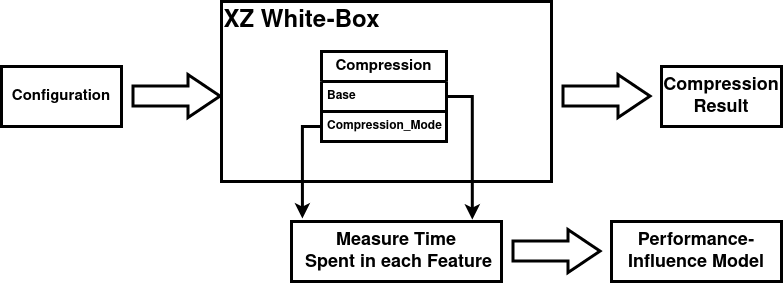
\includegraphics[scale=0.6]{gfx/whitebox_2.png}
    \caption{A white-box analysis of XZ}
    \label{fig:WBxz}
\end{figure}

We now analyze the example system from \autoref{fig:xz} using a white-box analysis. In \autoref{fig:WBxz} we can now see the inner workings of 
XZ when we are compressing a file. During the compression we can measure the time XZ spent in its various features, in our example we measure 
the time spent in $Base$ and $Compression_Model$, after system finished the process of compression we collected all measurements which we 
then use to build a \perfInfluenceModel for that configuration.

In this section we explain current state-of-the-art strategies and which principles they deploy to collect the measurements of each feature 
\ref{analyzing-strats}. We then proceed to explain which analyzing tool we use, a variability aware region analyzer and the underlying principles
behind it \ref{VaRA}. Afterwards we will aggregate the data that we collected to build a \perfInfluenceModel. % Ref TEF/Perf



%\subsection{Disadvantages of White-Box}
%When using white-box model we clearly see how a feature interacts with another feature, due to that we do not need to sample our configuration space like
%we do in the black-box, meaning we do not face the problem of combinatorial explosion. 
%Neither do we have to handle multicollinearity features differently, since we can see in what extend they influence each other. 
%The example from \ref{ColinearF} would be no problem for the white-box model since we are aware that $c$ and $d$ do not interact with one another and can
%therefore assign them the precise amount of time they spend in their code region respectively, whereas the black-box model needs to infer this information.

%With the surplus of information, the white-box model faces different challenges. 
%First and foremost, to analyze larger systems we need a robust strategy and in depth code comprehension.

\subsection{Analyzing Strategies}\label{analyzing-strats}
Analyzing programs is a highly complex topic in itself, it is not a trivial task to use a program to run an analysis over a different system.
In our case, we first need to find out which parts of the code corresponds to which feature.

To solve this problem multiple solutions have been proposed, Weber et. al. \cite{White-box-Profiling} uses a profiling approach, to generate 
performance-influence models that depict configurability on a method level, to achieve this they first used a JProflier a coarse-grained profiler
to learn a performance influence model for every method that have been learned successfully. 
To identify the methods that are hard to learn they use a filtering techniques, afterwards using KIEKER a fine-grained profiler to learn these methods.

Velez et. al. introduced us to ConfigCrusher \cite{ConfigCrusher} a white-box analysis, that uses a static data-flow analysis to see how features influence 
variables and the control-flow of the system. In addition, ConfigCrusher uses three insights about configurable systems, from previous works, namely
irrelevance, orthogonality and low interaction degree. Irrelevance, is used to identify the features that are relevant for the data-flow of the system, and by
doing so reducing the amount of configurations necessary to analyze the system. Orthogonality, is used to identify features that do not influence each other, and
thus can be measured together. Low interaction degree, is used to identify the relevant feature interaction, since only few features interact with another, 
ConfigCrusher focuses on those configurations with interacting features to reduce the amount of configuration that need to be sampled. 
Out of these insights two techniques are developed, namely compression and composition.
Compression is used to reduce the number of configurations necessary to analyze the system,
by simultaneously analyzing regions that are independent of another, therefore they can use a single configuration to 
analyze different features. 
They take advantage of the fact that \perfInfluenceModel can be build compositionally, by generating a performance-influcence model for each region separately
and afterwards compose all the local \perfInfluenceModel into a model for the whole system.

Siegmund et. al. introduced us to Comprex \cite{Comprex} which uses a dynamic taint analysis to identify how
and to what degree features influence the control-flow of the given system. 

Both Comprex and ConfigCrusher use the techniques of compression and composition, the major difference between both analysis methods is Comprex uses a dyanmic taint
analysis, whereas ConfigCrusher uses a static data-flow analysis, both are used to depict configurability on a feature level, where Weber et. al. depicts
configurability on a method level instead. 

After figuring out which parts of the code corresponds to what feature we still need to instrumentalize the code 

\subsection{VaRA}\label{VaRA}
To analyze the system we are interested in we use VaRA a variability aware region analyzer, a framework build on LLVM to analyze software
and the VaRA Tool Suite\footnote{Visited at 14.03.2022 \url{https://vara.readthedocs.io}}, developed at Saarland University. 

VaRA is able to 
detect which code regions are influenced by which feature using a data-flow analysis. Afterwards the code gets instrumentalized to measure the time
spent in each region. \cite{VaRA-Flo}

\subsubsection{VaRA Tool Suite}
We use VaRA in combination with the VaRA Tool-Suite which enables us to use VaRA by specifying an experiment to analyze a specific project. 

An experiment inside the VaRA Tool-Suite is a concept which specify how we want to analyze a software project, this allows us to make the analysis
easy to reproduce and repeat. The project specifies the system we want to analyze, here we  define how we build the system or which version we 
of the system we are interested in. 

For our example of \autoref{fig:WBxz}, the project would be XZ and would specify which version of xz we want to analyze and how the binary is build.
The experiment defines which configuration we want to analyze in addition to how we would like to analyze it, in our case we want to analyze 
XZ using VaRA, we also specify in what format we would like to have our measurements stored, such as the Trace Event Format in \ref{trace-event}.

\subsection{Trace Event Format}\label{trace-event}
When we analyze a system it is very rare that we only enter the region of a feature once and afterwards stop interacting with that feature. 